% Chapter 1
\chapter{Analysis} % Chapter title
\label{ch:analysis} % For referencing the chapter elsewhere, use \autoref{ch:architecture} 

%----------------------------------------------------------------------------------------

\section{Included and omitted functionalities}
On this section we will present which functions that have been created, are actually included in the website service and which are not due to various reasons. In the previous section, we describe the various phases of development of this project in detail. Despite the fact that all of the phases mentioned above have been fully developed, some functionalities have been unfortunately not included in the website application. This is mainly due to the limited amount of time at our disposal but also due to the amount of time required to include these functions in the application.\\

To begin with, we will briefly present what the application is capable of doing when used. When the user starts using the application, they upload an elevation model. Right after that, the application redirects them to a map with an overlaid image of the model they have uploaded. When that happens the user has to choose a point from where the flood will start. After doing that, they choose which type of flood they want to perform. The application then performs the chosen one and presents the results.\\

Now that we have stated what functions the application can perform, we will take a look on which functions have \emph{not} been included. To begin with, the first function concerns the barrier placement. On phase 4, we discuss in great extent the development of adding a barrier as a capability of the service. We also present in depth the problems we faced during the development of that functionality. In fact, this sub-process is fully developed and fully functional. Unfortunately, we have not managed to include it on our web-application so far. The reason is that we simply did not have the time to create the interface and connect the script to the server in order to allow the user to use that function to its full extent.\\

To go on, another function that is fully developed, tested and ready to use is the flood modeling with cost distance. The application is currently using the method spatial intersection. We have mentioned the reasons why we think that the cost distance modeling might be a better solution to simulating the flood. On the other hand, the cost distance method takes considerably more time to complete the entire process, especially if the user decides to use the advanced flood option. The changes that are needed in order to change from one method to the other are minimal, so if decided that the cost distance method is considerably better than the one currently in use, the switch to that method is fairly easy to make. \\  
Finally, the final function that we created but unfortunately was not included in the application was the outlet point identification. This process was created early in the development phases in order to locate points in the landscape where a bottleneck is created when the flood advances. Unfortunately, that approach did not perform as expected and the points that were identified did not contribute to the mitigation of the flood. For that reason, we decided that such process would not add to the overall efficiency of the application and as a result was discarded from the project.

\section{Architecture}
When the user visits the page, they have to provide a DEM, which has to fulfil the following criteria:

\begin{itemize}
\item Be a DEM
\item Have tiff image extension
\item Have WGS84 projection encoded
\end{itemize}

When this DEM is uploaded, and the source cell is selected, a request is sent to the server, by using PyWPS. PyWPS acts as a middleman, accepting the inputs from the user, initiating GRASS, and returning the results provided by GRASS encoded in a XML document. These results are then returned to the user through the browser, which are fetched and parsed using a combination of jQuery, JavaScript and HTML.

This overall workflow has been put into a diagram as can be seen on \autoref{fig:grass_archi}

\begin{figure}[h!]
\centering
	{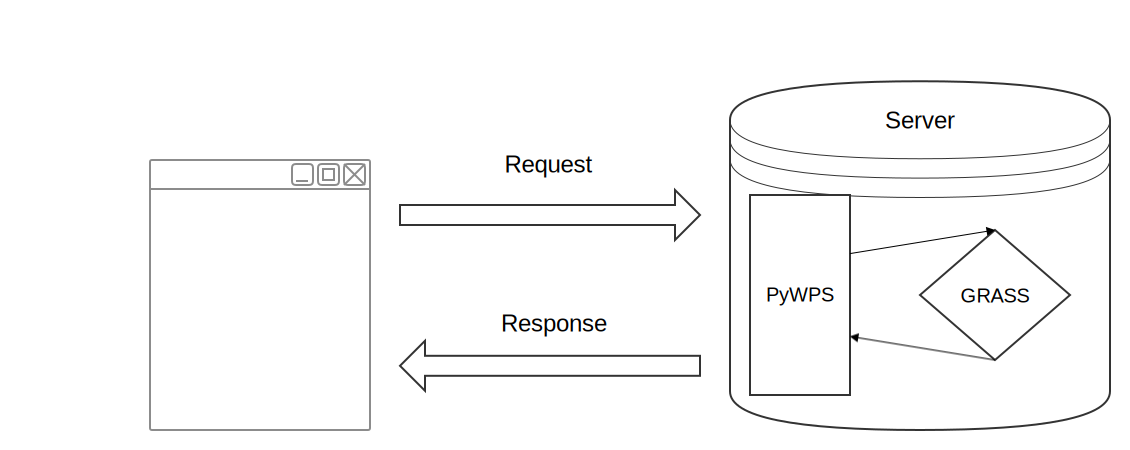
\includegraphics[width=\linewidth]{gfx/Analysis_Architecture/grass_pywps.png}}
\caption{The overall working of the application}
\label{fig:grass_archi}
\end{figure}

It should be noted however that, as mentioned in \autoref{ch:implementation}, we described the development of the functions implemented into the PyWPS service. As it turned out we created two different flooding models. One based on cost distance analysis, and one based on spatial selection. As mentioned in the problems encountered part of that section (\autoref{phase2problem}), we started out by developing the spatial selection method. As there was not time to fully implement the cost distance analysis method into the application, it is currently deployed to use the spatial intersection method.

\section{Installation structure}

Now that the application has been implemented, it is relevant to analyze how the entire installation is structured on the server. As mentioned in \autoref{ch:implementation}, a variety of software packages have been installed on the server, these being: 

\begin{itemize}
\item PyWPS
\item Flask
\item Apache2
\item GRASS
\end{itemize}

\paragraph{Debugging:} When the server has been installed, it runs on its own, and not much else has to be manipulated with, from then on. When the process fails for some reason, it can be relevant to troubleshoot the problem by reading the error log. Both Apache and PyWPS have error logs that can provide information about the situation, which can help to fix the error. The logs for both of these critical components can be found in the directories shown on \autoref{fig:anal_struct}:\\

\begin{figure}[h!]
\dirtree{%
.1 /.
.2 /var/.
.3 /www/.
.4 /html.
.5 /pywps/.
.6 pywps\.log.
.3 /log/.
.4 /apache2/.
.5 error\.log.
}
\caption{Location of the error logs.}
\label{fig:anal_struct}
\end{figure}

\paragraph{PyWPS installation:} When wanting to change or modify some of the functionality of PyWPS, it is necessary to access the server and perform the changes there. The setup is displayed in \autoref{fig:pywpsinstall}. 

\begin{figure}[h!]
\dirtree{%
.1 /.
.2 /var/.
.3 /www/.
.4 /html.
.5 /pywps/.
.6 pywps\.log.
.6 pywps.cfg.
.6 /processes/.
.7 \_\_init\_\_.py.
.7 process1\.py.
}
\caption{Structure of the PyWPS installation.}
\label{fig:pywpsinstall}
\end{figure}

When adding or removing processes, it has to be done in the processes folder. The process is added (or removed) from the drive, and the \_\_init\_\_.py file is modified to reflect the change that has occurred in the drive.

A variety of serverside settings can be managed from the pywps.cfg file, for instance the maximum allowed filesize of a DEM used as input, or the location of PyWPS outputs.

\paragraph{Flask installation:}Flask is installed in the directories shown on \autoref{fig:flaskinstall}.\\

\begin{figure}[h!]
\dirtree{%
.1 /.
.2 /var/.
.3 /www/.
.4 /html.
.5 /FlaskApp/.
.5 flaskapp\.wsgi.
.6 /FlaskApp/.
.7 /templates/.
.7 /images/.
.7 /static/.
.7 \_\_init\_\_.py.
}
\caption{Installation structure of Flask}
\label{fig:flaskinstall}
\end{figure}

It is within the \_\_init\_\_.py file that most changes mentioned in the Implementation section have been performed. The templates folder contains the templates used to display HTML. The static folder contains a variety of static content, such as the jQuery and CSS libraries. A functionality of Flask is that content on the server that is not directly served to the user, is not meant to be accessible. But if it is placed within the static folder, and the URL to the content is known, it can be accessed from “outside”. The outputs of the PyWPS service are therefore directed to a subdirectory of the static folder, so that we can easily access the data through the website front-end.
The images folder is used to store the DEM the user uploads and works with, through the entire process.\\

\paragraph{GRASS Installation:}The GRASS installation is fairly simple (and the structure can be seen in \autoref{fig:grassinstall}), and after the initial setup is not touched even when adding new functionalities. The \textit{grassdata} folder normally contains the various locations and mapsets that are used by the user. In our case the folder only contains one LOCATION, using the WGS84 geographical reference system. This will be used by the PyWPS process to work with the data in question. 
The \texti{.grassrc6} folder contains some settings that are needed for GRASS to function properly.

\begin{figure}[h!]
\dirtree{%
.1 /.
.2 /home/.
.3 /ubuntu/.
.4 \.grassrc6.
.4 /grassdata/.
.5 <LOCATION>.
.6 <MAPSET>.
}
\caption{Installation folder structure of GRASS}
\label{fig:grassinstall}
\end{figure}

\section{User experience}
In this part of the report we will present  how our web service works from the point of view of the user. What we will do, is try to demonstrate as detailed as possible the actual results of the phases we described on the previous chapter. We will also include a step-by-step guideline on how the service should be used and what actions are necessary for the user to follow in order to get the best results possible out of this process. But before we go in depth of the structure of the website, we will take a look at the overview of the setup, as seen on \autoref{fig:analysis_1}

\begin{figure}[h!]
\centering
	{\includegraphics[height=0.33\textheight]{gfx/Analysis_Website/1.jpg}}
\caption{Overall workflow of the application}
\label{fig:analysis_1}
\end{figure}

We begin by presenting the first page the user will see when they visit our website \autoref{fig:analysis_frontpage}. The url that leads to the homepage of the application is \url{http://52.17.144.192/}. The first page is then displayed, this provides information about the website such as its name and a basic description of what services it offers (\autoref{fig:analysis_2}.

\begin{figure}[h!]
  \myfloatalign
  \subfloat[Banner.]
  {\label{fig:analysis_2}  
  {\includegraphics[width=\linewidth]{gfx/Analysis_Website/2.png}}} \quad
  \subfloat[Banner]
  {\label{fig:analysis_3}  
  {\includegraphics[width=0.45\linewidth]{gfx/Analysis_Website/3.png}}} \quad
  \subfloat[Middle.]
  {\label{fig:analysis_4}%
   \includegraphics[width=0.45\linewidth]{gfx/Analysis_Website/4.png}} \\
 \caption{Frontpage of the web application, tentatively dubbed \textit{flooding}.}
 \label{fig:analysis_frontpage}
\end{figure}

Lower on the same page, we provide the user with detailed information about the application; The reason we have created it; who can use it; its most important advantages and features \autoref{fig:analysis_3}

On the final part of the page, we provide the user with small examples of the programming languages, frameworks and other tools we used on order to create this service (\autoref{fig:analysis_4})

In order to proceed with the actual simulation the option FLOOD on the first part of the page has to be chosen. That will create a new tab on the browser that leads to the second part of the website (\autoref{fig:analysis_upload}). This part is a guided process of the flood simulation that follows. By clicking on commence flooding option, the initial part of the flood commences.

\begin{figure}[h!]
  \myfloatalign
  \subfloat[Page describing the coming process.]
  {\label{fig:analysis_2}  
  {\includegraphics[width=\linewidth]{gfx/Analysis_Website/5.png}}} \quad
  \subfloat[Uploading a DEM.]
  {\label{fig:analysis_3}  
  {\includegraphics[width=\linewidth]{gfx/Analysis_Website/6.png}}} \quad
 \caption{Accessing the possibility of uploading a DEM.}
 \label{fig:analysis_upload}
\end{figure}

The process starts with requesting the user for the necessary input in order for the application to run (\autoref{fig:analysis_3}). As mentioned in previous parts of the report, that necessary input is an elevation model. 

Once the user chooses an elevation model from his local hard drive and then uploads it, the second step is initialized (\autoref{fig:analysis_7}). 


\begin{figure}[h!]
\centering
	{\includegraphics[width=0.80\linewidth]{gfx/Analysis_Website/suckmycock.PNG}}
\caption{Step 2 display uploaded elevation model and insert point to designate origin of flood}
\label{fig:analysis_7}
\end{figure}

Afterwards the user is required to provide it with the source of the flood. By simply clicking on the map, that point is created. 
Finally, the user then has to decide which type of process they wish to perform. The simple flood option will instantly fill the elevation model with a predefined level of water and display the results on a map on the third step (\autoref{fig:analysis_8}).

\begin{figure}[h!]
\centering
	{\includegraphics[width=\linewidth]{gfx/Analysis_Website/8.png}}
\caption{Results of the simple flood option}
\label{fig:analysis_8}
\end{figure}

The advanced flood will return the same flood extent, with the pour points returned as vector points. 

\section{Old vs New model}
As discussed in \autoref{ch:phase2}, we have tried to simplify the model as much as possible, using only simple geoprocessing tools and map calculator. However here we would like to mention, since we used only ArcMap Model Builder in the old version, the coding part behind that model will not be taken into this comparison.

\paragraph{The old workflow:} The old model had been set up with two consecutive parts. An input part of the model, that specified the required input for the further modelling, such as input point for source selection and maximum flood level. As seen in \autoref{fig:arcgismodel}, the input part of the model, consists of a series of different modules.  ArcGIS ModelBuilder is useful when constructing and executing simple workflows, and also has the functionality enabling it to export the created model to python script, however the python script conversion will disregard most of the environment setting and iteration functions. Therefore it is only useful as a preliminary decision making tool for developing a model.

\begin{figure}[h!]
  \myfloatalign
  \subfloat[Input part of the old model.]
  {\label{fig:arcgisa}
  {\includegraphics[width=0.75\linewidth]{gfx/Analysis_OldWork/1.png}}} \\ \quad
  \subfloat[Flooding iteration of the old model.]
  {\label{fig:arcgisb}
   \includegraphics[width=0.75\linewidth]{gfx/Analysis_OldWork/2.png}} \\
  \caption{ArcGIS modelbuilder workflow of old model.}
  \label{fig:arcgismodel}
\end{figure}

Our ArcGIS model, however it was functioning perfectly, it was slightly harder to track down the errors, when the process executed with a lot of iteration. Also, the whole workflow was separated into two parts because you cannot iterate a part of a model, which means that another process needs to be involved in workflow, that part needs to incorporated into a separate model. Because of this, input variables for the flood modeling were defined in the first part of the workflow, and were passed a second model containing the flooding modelling part.

\paragraph{The new model}

As described in \autoref{ch:implementation} we simplified the model as much as possible, by taking out most of the unnecessary processes. During the development we have created a series of extensions for our flood model, however only the pour point analysis has been deployed to the server, due to the lack of time. As can be seen in \autoref{fig:grasspython}, the workflow consists of the barrier process, however it has not been included in the deployed script, but it has been developed and is working correctly.

If we are comparing the two workflows (old and new), it is clearly visible how much the simplification has impacted on the process. The iteration process is clearer and more straight forward. Also here we can mention, that our ArcGIS model was a very good model, however it is not suitable for distribution, since we do not have the right to publish the modules on an online service, as it can cause copyright issues. 

\begin{figure}[h!]
\centering
	{\includegraphics[width=\linewidth]{gfx/Analysis_OldWork/3.jpg}}
\caption{The new GRASS python model.}
\label{fig:grasspython}
\end{figure}\\

\paragraph{New model vs results from COWI:} As in our last project, we have compared our flood extent results with COWI data, who have created a delineation based on the flood aftermath of the storm Bodil in 2013. COWI calculated that the flood extent will appear as shown on \autoref{fig:cowi}. This stage appears at level 165 cm, and it can be seen that the water accessed the residential area through from the North and furthermore a channel formed from the West, which can lead the accumulated water further.

\begin{figure}[h!]
\centering
	{\includegraphics[width=\linewidth]{gfx/Analysis_OldWork/COWI.jpg}}
\caption{COWI flood extent.}
\label{fig:cowi}
\end{figure}

\begin{figure}[h!]
  \myfloatalign
  \subfloat[Cost distance model flooding.]
  {\label{fig:cdflood}
  {\includegraphics[width=0.45\linewidth]{gfx/Analysis_OldWork/4.png}}} \quad
  \subfloat[Spatial selection model flooding.]
  {\label{fig:spatialselectflood}
   \includegraphics[width=0.45\linewidth]{gfx/Analysis_OldWork/5.png}} \\
  \caption{Output of the GRASS modelling approaches.}
  \label{fig:cdandspatialflood}
\end{figure}

As described in Phase 2, we have created an approach for flood extent delineation with spatial selection and cost distance analysis. Comparing our flood stages with the COWI flood, we realized that our calculated extent is the same, however the above presented extent appears at stage 174 cm with our Cost Distance model \autoref{fig:cdflood}. The model with spatial selection (\autoref{fig:spatialselectflood}) could reach this stage at 175 cm, therefore we can state that the deviation between the two models is relatively low. 

\section{Limitations}
In this section, we will discuss the existing limitations the users might face while using our application. These limitations are either placed by us, to ensure that our application works at an optimal level or exist purely because of the features and the parts that consist it. Regardless of the origins of these limitations, we think that it is our responsibility to let the user know about them and notify them before using the application, so that we can save them time while using it.

\paragraph{Extensions and filename:} The first limitation we set is during the uploading of the input by the user. In an effort to apply some sort of control on what the user is capable of uploading to our server, we made sure that only certain file types are allowed for upload. The reason behind this specific action is that we do not want to allow irrelevant files on our server. Mainly because we want to make sure that the memory of the server is reserved for files that are actually compatible with the application but also install a first wall of security against malicious intents. That being said, the user can only upload \textit{.tif} files. This file type check is performed in two steps. First, we declare the types that are allowed for upload.

\begin{lstlisting}
ALLOWED_EXTENSIONS = set(['tif'])
\end{lstlisting}

Then we create a function that checks the extension of a file-to-be uploaded and if it is included in the ALLOWED EXTENSIONS, basically a tiff file, it returns a true  value:

\begin{lstlisting}
def allowed_file(filename):
	return '.' in filename and \
			filename.rsplit('.',1)[1] in ALLOWED_EXTENSIONS
\end{lstlisting}

Finally, we set a condition that checks the result of the function mentioned above and if it is true, then it proceeds with uploading the file, otherwise it will reload the upload page without any results

\begin{lstlisting}
#check if the extension is allowed
if allowed_file(file.filename):
\end{lstlisting}

Having said that, the main reason we decided to use tiff as the only allowed extension the uploaded file can have is because tiff files contain necessary spatial information of the file. To be more precise, important information about the geographical reference system, the projection in use and the coordinates of the file's bounding box are all contained within tiff file. This is the main reason we set this file extension as the only one allowed and do not include for example \textsc{ascii} files that need an additional file that holds some of the important geographical reference system information.\\

Another limitation we have implemented concerns the name of the file. This is because we want to make sure that  our server is secure from malicious files that may be able to affect our server in any way through their filename.

\paragraph{Nodata value:} Since we have established what kind of limitations exist based on the file that the user wishes to upload, we will now examine how the file itself can obstruct the user from using our application properly. 
One obstacle that can result in a critical failure of the application exists when the user selects a point to designate water in the uploaded file. To be more specific, when the user uploads a file, that file is converted to \textit{.png} in order to overlay it on the map and display it. That affects the way nodata cells are represented. Normally, when examining a \textit{.tif} file, the cells that have null values are easily distinguished
On the other hand, \textit{.png} formatted files cannot display null valued cells as shown on \autoref{fig:analysis_nodata}.

\begin{figure}[h!]
\centering
{\includegraphics[width=0.8\linewidth]{gfx/Analysis_Specs/nodata.png}}
\caption{Image showing NoData values in tiff image.}
\label{fig:analysis_nodata}
\end{figure}

Since this is a case when displaying a \textit{.png}, the user must be very careful when choosing the origin of the flood because if the coordinates of the point are within an area of null values, then the application will produce an error.

\paragraph{Cell values for water:} One of the core prerequisites our application that needs to be fulfilled is the designation of the water cells. Apart from the point that the user must provide to the application, the file that the user wants to investigate has to have cells that represent the sea. What we mean by that is that the representation of the sea is not consistent across every elevation model worldwide. For example, the Danish DEM represents sea and water in general with zero values. Other elevation models do the same with negative values. Finally, some also do not use any kind of representation of the water resulting in them being shown as null cells for example NASA's Shuttle Radar Topography Mission (SRTM). As far as the negative values are concerned, it does not present as a problem because the way we have developed the application, all cells that are equal or lower than zero are considered as water. In the case where water is not represented, then the application will not work at all, in a similar manner with the nodata box described above.

\section{Audience}
Throughout this report we have mentioned in detail the characteristics of the application: its requirements to function properly, the decisions that need to be made in order for it to produce reliable results and the problematic parts of it that require attention in order to avoid erroneous results. Taking all of the above into consideration, we have concluded on a group of people that not only will find this application useful, but will also know how to use it to its full extent and potential.\\
Surely, the product of our work is not meant to be operated by everyone, even though that would be quite desirable. There is a limit on which people can operate our product in an efficient manner and that fact comes from the various components that were needed in order to create such application. A lot of considerations that we have made are so in order to ensure that our application is available to the widest possible audience. Unfortunately, there are elements that for better or worse, limit that audience.\\

To begin with, we believe that the setup and interface of the application is as straightforward as possible. That ensure that it is easy to use and understand by anyone. As the user goes on in the application that changes. When we require the user to upload an image, then he/she needs to understand that the application performs at its fullest when provided with an elevation model that uses the WGS84 geographical reference system. That fact alone, requires some amount of knowledge in the fields of geography, surveying or cartography.\\

Another limiting factor is the actual input of the application. As presented above, the elevation model is the most important input the user has to provide. After the upload the user will then designate the source of the flood. As presented above, that approach requires great attention because an erroneous selection of the flood source can result in failure of the process. This entire process of designating the flood and making sure that the source point is within the extent of the raster requires a certain acquired experience with working with rasters. \\
Finally, another deciding factor that sets limitations on who can use this application is the hydrologic aspect of it. This aspect concerns the evolution of the flood event, its spread across the landscape as well as the management of the event. To be more specific, we believe that in order to use this tool at its maximum extent and produce reliable results and create efficient solutions, the user would probably need to have some experience with hydrology. That is because the tool uses a number of terms from that field in order to produce the results it does and understanding these terms and how they affect the results of the process is important to design viable solutions.
